% Size class quick reference: adding a new size class to the size class file, on one page.
% One 11 x 17 landscape sheet (ledger, 17 x 11 in) in TikZ: sheet 5 of size-class-file-guide.tex on its own, without
% the orange frame and banner (it is the only page), the title naming the file and the macro it belongs to.
% The file: output/open-orders-intake-inventory/size-class-master.xlsx (Config setting SizeClassFile of the
% Open Orders by MSA report macro, build-open-orders-report.bas v2.8). Pictures from size-class-guide/, written by
% make_size_class_guide_shots.py (example classes shaded peach in the pictures only). Keep the steps in step with
% sheet 5 of the guide.
% The sheet is laid out on a 12 x 7.5 in grid and scaled by 4/3 to fill the 16 x 10 in drawing area.
% Build: ./build.sh source/open-orders-intake-inventory/size-class-quick-reference-v1-2026-10-16.tex
\documentclass[10pt]{article}
\usepackage[paperwidth=17in, paperheight=11in, margin=0.5in]{geometry}
\usepackage[T1]{fontenc}
\usepackage{lmodern}
\usepackage{microtype}
\usepackage{enumitem}
\usepackage[table]{xcolor}
\usepackage{graphicx}
\usepackage{tikz}
\usetikzlibrary{positioning, arrows.meta, calc, fit}
\usepackage[hidelinks, pdftitle={Size Class Quick Reference}, pdfauthor={Gust F.}]{hyperref}
\graphicspath{{size-class-guide/}}
\pagestyle{empty}
\setlength{\parindent}{0pt}
\hyphenpenalty=10000
\exhyphenpenalty=10000
\setlist[itemize]{label=\textbullet, leftmargin=0.85em, labelsep=0.35em, itemsep=1.5pt, parsep=0pt,
                  topsep=0pt, partopsep=0pt}
\definecolor{headgreen}{HTML}{548235}
\definecolor{bandgreen}{HTML}{E2EFDA}
\definecolor{flagpeach}{HTML}{FCE4D6}
\definecolor{inputyellow}{HTML}{FFFFCC}
\tikzset{
  every node/.style={font=\sffamily\small, inner sep=5pt},
  box/.style={draw, line width=0.5pt, fill=white, align=left},
  station/.style={draw, line width=0.5pt, fill=headgreen, text=white, font=\sffamily\bfseries\normalsize,
                  align=left, inner ysep=4pt, text height=1.6ex, text depth=0.45ex},
  flow/.style={-{Stealth[length=9pt, width=6.5pt]}, line width=1.2pt, line join=miter},
  point/.style={-{Stealth[length=6pt, width=4.5pt]}, line width=0.9pt, headgreen},
  % a numbered marker on a picture, matched by the same number in the text beside it
  marker/.style={circle, fill=headgreen, text=white, draw=white, line width=1pt, font=\sffamily\bfseries\small,
               inner sep=0pt, minimum size=0.25in},
  shot/.style={draw, line width=0.5pt, inner sep=0pt, anchor=north west},
}
\newcommand{\by}[1]{{\footnotesize\itshape #1}\\[3pt]}
\newcommand{\peach}[1]{{\setlength{\fboxsep}{1pt}\colorbox{flagpeach}{\textbf{#1}}}}
\newcommand{\yellow}[1]{{\setlength{\fboxsep}{1pt}\colorbox{inputyellow}{#1}}}
\newcommand{\btn}[1]{{\setlength{\fboxsep}{1.5pt}\fbox{\footnotesize\bfseries #1}}}
\newcommand{\num}[1]{\tikz[baseline=(n.base)]\node(n)[marker, minimum size=0.2in, font=\sffamily\bfseries\footnotesize]{#1};}
\newcommand{\cls}[1]{{\ttfamily #1}}
% title block, one row in the bottom right corner: #1 title, #2 sheet
\newcommand{\titleblock}[2]{%
  \draw[line width=0.5pt] (5.7,0) -- (5.7,0.42) -- (12,0.42);
  \foreach \x in {7.3, 8.95, 9.5, 9.95, 10.75, 11.45} \draw[line width=0.5pt] (\x,0) -- (\x,0.42);
  \foreach \x/\label/\value in {5.7/Title/#1, 7.3/Project/Open Orders by MSA, 8.95/Macro/v2.8, 9.5/Rev./1,
                                9.95/Date/2026-10-16, 10.75/Drawn/Gust F., 11.45/Sheet/#2} {
    \node[anchor=north west, inner sep=0pt, font=\sffamily\fontsize{7}{8}\selectfont] at (\x+0.07,0.36) {\label};
    \node[anchor=south west, inner sep=0pt, font=\sffamily\bfseries\footnotesize] at (\x+0.07,0.07) {\value};
  }}
% sheet heading: #1 title, #2 subtitle
\newcommand{\heading}[2]{%
  \node[anchor=north west, inner sep=0pt, font=\sffamily\bfseries\fontsize{14}{16}\selectfont] at (0.25,7.25) {#1};
  \node[anchor=north west, inner sep=0pt, font=\sffamily\footnotesize] at (0.25,6.88) {#2};}

\begin{document}
% ============================================================================ the quick reference
% pictures: setup-after 2062 x 1116 px, 6.6 in wide, so 3.572 in high, top left at (5.15,6.0);
%           size-class-new 1907 x 395 px, 6.6 in wide, so 1.367 in high, top left at (5.15,1.95)
\noindent
\scalebox{1.333333}{%
\begin{tikzpicture}[x=1in, y=1in]
\useasboundingbox (0,0) rectangle (12,7.5);
\draw[line width=0.8pt] (0,0) rectangle (12,7.5);
\node[anchor=north west, inner sep=0pt, font=\sffamily\bfseries\fontsize{14}{16}\selectfont]
  at (0.25,7.25) {Quick Reference: Add a New Size Class (CTL, SSL, MX) to \texttt{size-class-master.xlsx}};
\node[anchor=north west, inner sep=0pt, align=left, font=\sffamily\footnotesize] at (0.25,6.9)
  {The size class file of the Open Orders by MSA report macro (\texttt{build-open-orders-report.bas} v2.8; Config setting
   \texttt{SizeClassFile}). It sets the size class of every model in the report.\\[2pt]
  The same steps for all three families; only the table changes. Example: \cls{4000\&Over} (CTL), \cls{XL Frame} (SSL),
   \cls{>10-15} (MX), shaded \peach{peach} in the pictures. Use the class names your size class slide gives.};

% ---------------------------------------------------------------- the steps
\node[station, anchor=north west, text width=4.45in] (s1) at (0.25,6.45) {\num{1}\enspace Open the file, go to the Set-up tab};

\node[station, anchor=north west, text width=4.45in] (s2) at ($(s1.south west)+(0,-0.12)$) {\num{2}\enspace Find the table of the family};
\node[box, anchor=north, text width=4.45in, font=\sffamily\footnotesize] (t2) at (s2.south) {%
  \renewcommand{\arraystretch}{1.2}%
  \begin{tabular}{@{}p{0.5in}p{1.5in}p{0.7in}p{1.3in}@{}}
  \textbf{CTL} & Table 1 & column \textbf{A} & e.g.\ \cls{4000\&Over} \\
  \textbf{SSL} & Table 2 & column \textbf{C} & e.g.\ \cls{XL Frame} \\
  \textbf{MX}  & Table 3 & column \textbf{E} & e.g.\ \cls{>10-15} \\
  \end{tabular}};

\node[station, anchor=north west, text width=4.45in] (s3) at ($(t2.south west)+(0,-0.12)$) {\num{3}\enspace Type the class in the first empty yellow cell};
\node[box, anchor=north, text width=4.45in] (t3) at (s3.south) {%
  \begin{itemize}
  \item Spell it as the report should show it; one class per cell
  \item Largest class? It goes at the bottom, as in the example
  \item Belongs between two classes? Select the cells from that spot down to the last class, drag their
        border one cell down, then type in the gap. Never insert whole rows
  \end{itemize}};

\node[station, anchor=north west, text width=4.45in] (s4) at ($(t3.south west)+(0,-0.12)$) {\num{4}\enspace Check Table 4 (column G)};
\node[box, anchor=north, text width=4.45in] (t4) at (s4.south) {%
  The new class shows in its place in the list: it is now in the drop-down.};

\node[station, anchor=north west, text width=4.45in] (s5) at ($(t4.south west)+(0,-0.12)$) {\num{5}\enspace Give it to the models, on the Size Class tab};
\node[box, anchor=north, text width=4.45in] (t5) at (s5.south) {%
  Pick the new class in column D for each model in it; a new model goes in the first empty row (Name of machine in column C, as the export spells it). Save and close.};

\node[station, anchor=north west, text width=4.45in] (s6) at ($(t5.south west)+(0,-0.12)$) {\num{6}\enspace Config: \btn{Check setup}, then \btn{Build report}};
\node[box, anchor=north, text width=4.45in] (t6) at (s6.south) {%
  The Run Log counts the new classes (the example):
  {\footnotesize\ttfamily Size classes: 20 from the Set-up tab (CTL 7, MX 8, SSL 5)}};

% ---------------------------------------------------------------- the Set-up tab after step 3
\node[anchor=south west, inner sep=0pt, font=\sffamily\bfseries\small] at (5.15,6.08) {Set-up tab after step 3};
\node[shot] at (5.15,6.0) {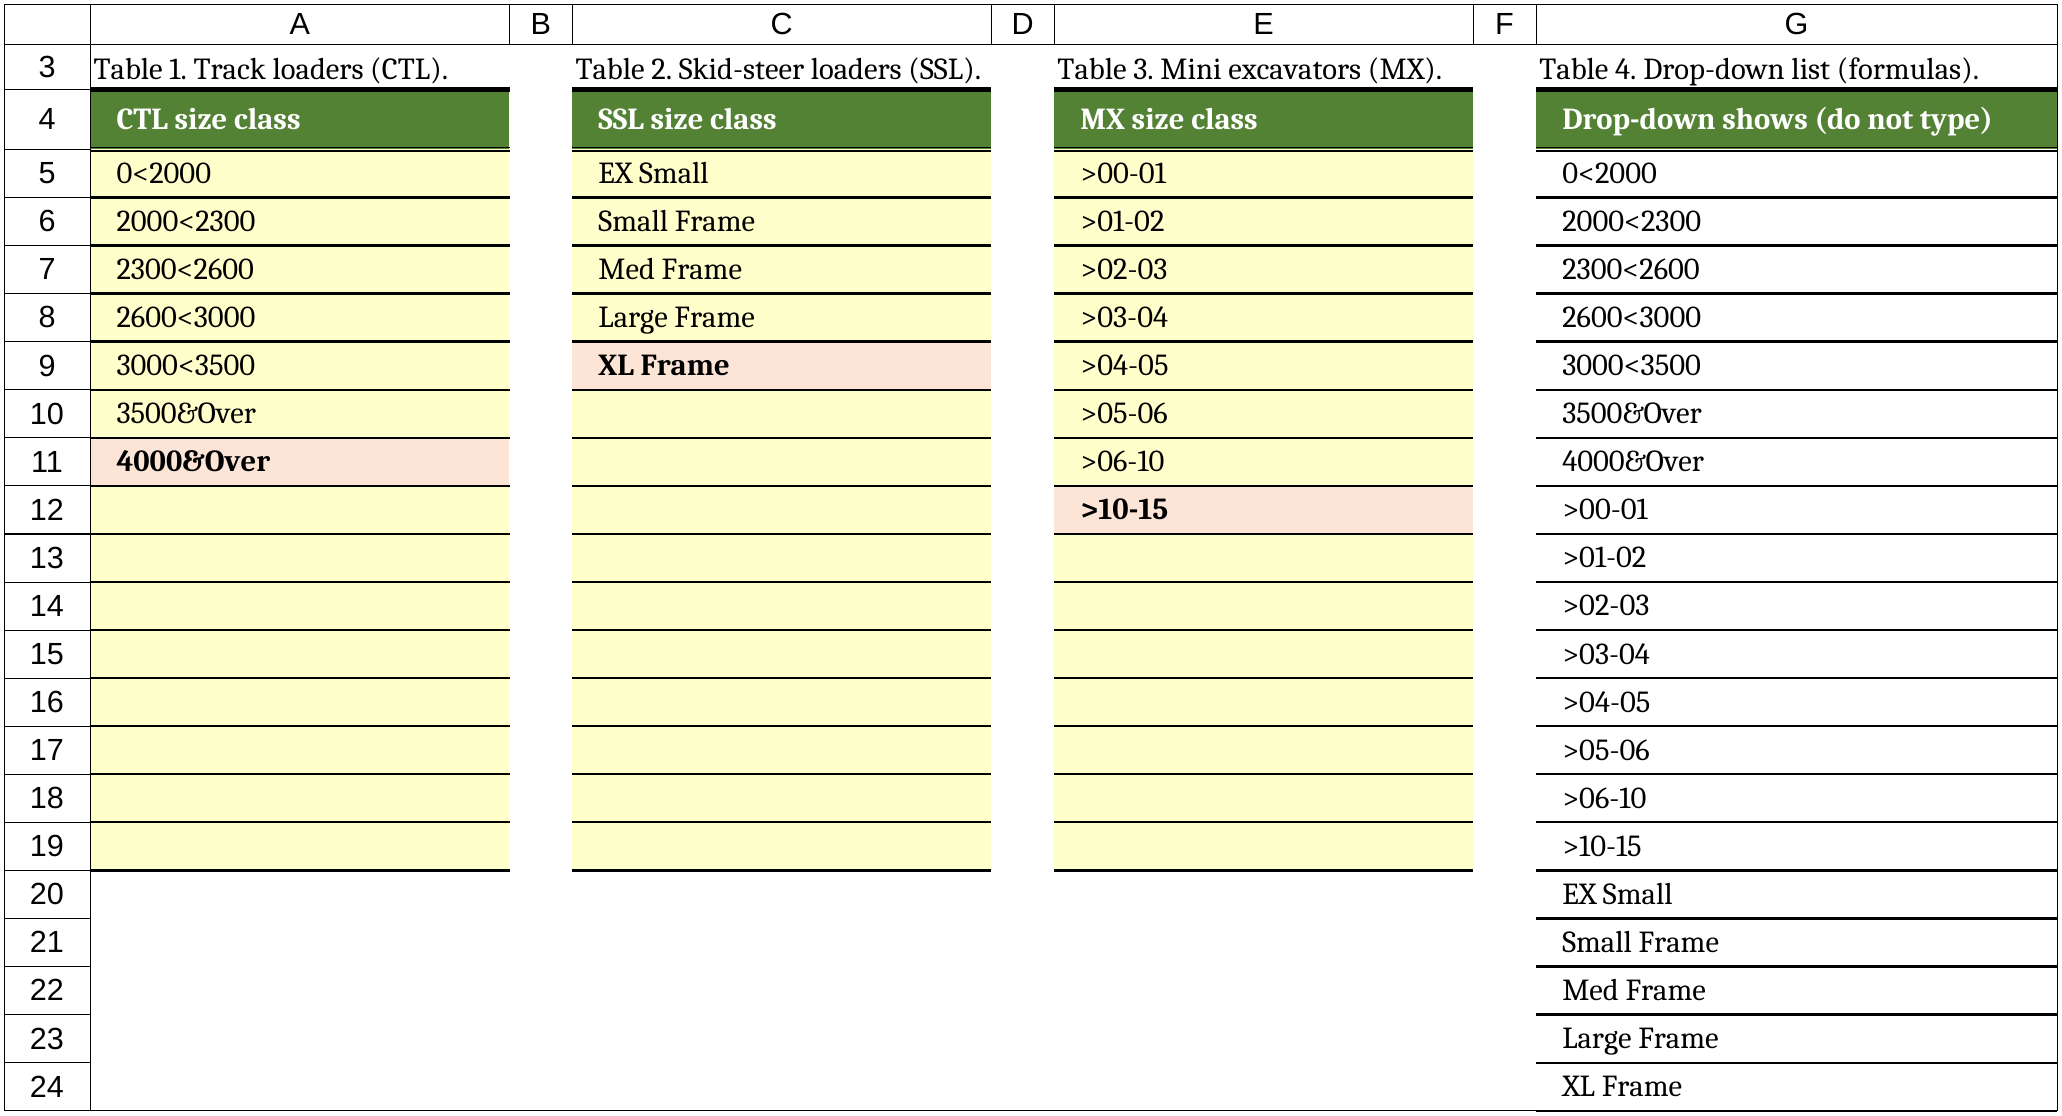
\includegraphics[width=6.6in]{setup-after.png}};
\begin{scope}[shift={(5.15,6.0)}, x=6.6in, y=-3.572in]
  % step 3: the three cells typed (A11, C9, E12)
  \node[marker] at (0.215,0.412) {3};
  \node[marker] at (0.448,0.327) {3};
  \node[marker] at (0.681,0.456) {3};
  % step 4: where they show in Table 4 (G11, G19, G24)
  \foreach \fy in {0.412, 0.757, 0.972} \draw[line width=1.4pt, headgreen] (0.745,\fy-0.021) rectangle (0.995,\fy+0.021);
  \node[marker] at (0.70,0.757) {4};
  \foreach \fy in {0.412, 0.757, 0.972} \draw[point] (0.70,0.757) ++(0.012,{0.02*sign(\fy-0.757)}) -- (0.743,\fy);
\end{scope}

% ---------------------------------------------------------------- the Size Class tab after step 5
\node[anchor=south west, inner sep=0pt, font=\sffamily\bfseries\small] at (5.15,2.03) {Size Class tab after step 5 (header and last rows)};
\node[shot] at (5.15,1.95) {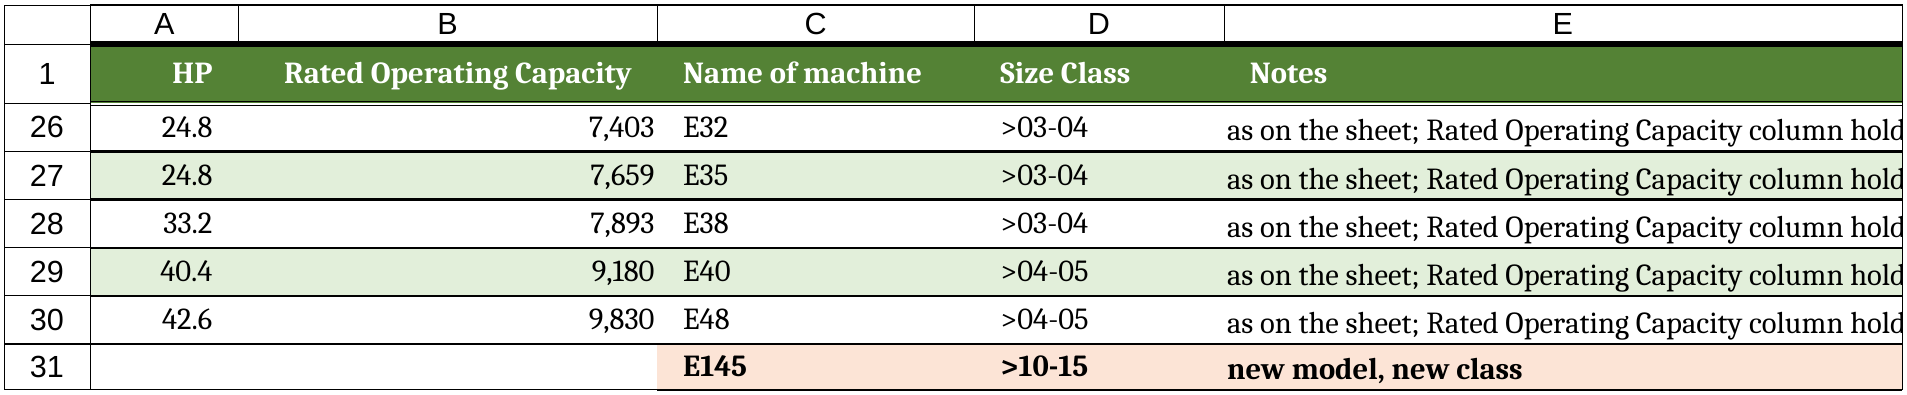
\includegraphics[width=6.6in]{size-class-new.png}};
\begin{scope}[shift={(5.15,1.95)}, x=6.6in, y=-1.367in]
  \node[marker] at (0.495,0.927) {5};
\end{scope}

% ---------------------------------------------------------------- the don'ts
\node[anchor=north west, draw, line width=0.5pt, fill=flagpeach, text width=4.45in, align=left, font=\sffamily\footnotesize]
  at ($(t6.south west)+(0,-0.2)$) {\textbf{Do not:} type in Table 4, change the green headers, insert or delete whole rows,
  or type a class twice or the word UNMAPPED. Up to 15 classes per table.};

\titleblock{Quick Reference}{1 of 1}
\end{tikzpicture}}
\end{document}
